\documentclass[12pt, a4paper]{article}

\usepackage{comment}
\usepackage{ragged2e}
\usepackage{amsmath}
\usepackage{dcolumn}
\usepackage{booktabs}
\usepackage{pdflscape}
\usepackage{graphicx}
\usepackage{placeins}
\usepackage{dcolumn}
\usepackage{xcolor}
\usepackage{booktabs}
\linespread{1.5}
\usepackage{subcaption}
\usepackage{amsmath}
\usepackage{hyperref}
\usepackage{multirow}
\usepackage{tikz}
\usepackage[title]{appendix}
\usetikzlibrary{decorations.pathreplacing}
\usepackage{booktabs}
\usepackage{tabularx}
\usepackage{datatool}
\hypersetup{
	colorlinks=false,
	linkcolor=black,
	filecolor=black,      
	urlcolor=black,
	citecolor = blue
}

\usepackage{natbib}
\usepackage{xepersian}
\settextfont{XB Niloofar}
\setdigitfont{XB Zar}
\newcommand{\paren}[1]{\scaleleftright[3cm]{\text{)}}{#1}{\text{(}}}
\def\sym#1{\ifmmode^{#1}\else\(^{#1}\)\fi}

\title{مالکان نهایی و هم‌زمانی بازده شرکت با بازار}
%\subtitle{}
\author{
	مرتضی آقاجان‌زاده
	 \sym{*} 
	\qquad 
	مهدی حیدری 
	\sym{*} 
	 \\
	\sym{*} 
	\footnotesize  موسسه مطالعات پیشرفته تهران (تیاس) - دانشگاه خاتم
}

\date{
تیر 1400}




\begin{document}

\maketitle

\section{مقدمه}
\section{پیشینه پژوهش}
\section{روش‌شنای پژوهش}
\subsection{هم‌زمانی بازده شرکت}
معولا در ادبیات هم‌زمانی بازده شرکت را با ضریب تعیین برآورد خطی بازده شرکت بر روی بازده بازار و صنعت شرکت محاسبه می‌کنند. هر آنچه یک شرکت دارای ضریب تعیین بالاتری باشد، بازده شرکت با بازده بازار و یا صعنت هم زمانی بالاتری دارد. 
با توجه به مقاله 
پیتروسکی و رولستون (2004)
%\lr{\cite{piotroski2004influence} }
به منظور بدست آوردن هم زمانی قیمت سهام، معادله زیر را برای هر شرکت به صورت سالانه برازش می‌کنیم:
	\begin{equation}\label{e1}
		RET_{i,w} = \alpha + \beta_1 MKRET_{w}+ \beta_2 MKRET_{w-1}  + \beta_3 INDRET_{i,w} + \beta_4 INDRET_{i,w-1} 
	\end{equation}
	که در این معادله 
	\lr{$ RET_{i,w} $}
	بازده هفتگی شرکت i در هفته w، 
	\lr{$ MKRET_{w} $}
	بازده بازار برای هفته w و
	\lr{$ INDRET_{i,w} $}
	بازه صنعت شرکت در هفته w می‌باشد که بازده شرکت مورد بررسی از آن کم شده‌است. 
	
	ضریب تعیین بدست آمده از برازش فوق عددیدر بازه یک و منفی یک می‌باشد به همین علت نمی‌توانیم از آن به صورت مستقیم در برآورد‌های آینده استفاده کنیم. به همین منظور از تبدیل لاجستیک استفاده می‌کنیم. در نتیجه متغیر اصلی هم‌زمانی بازده شرکت برابر است با 	
	\begin{equation}
		SYNCH_{i,t} = log(\frac{R^2_{i,t}}{1-R^2_{i,t}})
	\end{equation}
که در این عبارت $  R^2_{i,t}$ ضریب تعیین بدست آمده از برازش معادله 
\ref{e1}
برای شرکت
 \lr{i}
  و در سال
 \lr{ t}
  می‌باشد. در شکل
  \ref{fig:synchtimeseries} 
  سری زمانی هم‌زمانی بازده برای تمامی شرکت‌های حاضر در بازار رسم شده‌است. به صورت متوسط مقدار هم‌زمانی بازده در بازار ایران برابر
$    0.62 $
   می‌باشد که از مقادیر کشور‌های توسعه یافته به مراتب بیشتر است (برای مثال در بازار آمریکا  و فرانسه به ترتیب این مقدار برابر
   $    -1.75  $ , $ -1.22 $
   می‌باشد) و این به معناست که در بازار ایران  نسبت به کشور‌های توسعه یافته قیمت شرکت‌ها بیشتر از اطلاعات بازار و صنعت ناشی می‌شود.   در ادبیات نیز به این نکته اشاره شده‌است که در کشور‌های در حال توسعه مقدار هم‌زمانی بازده نسبت به کشور‌های توسعه یافته بیشتر است که یافته‌های این پژوهش نیز این امر را تایید می‌کند.
  
  
  \begin{figure}[htbp]
  	\centering
  	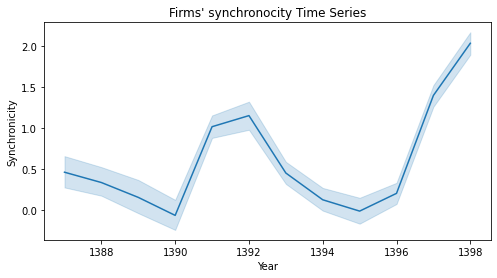
\includegraphics[width=0.85\linewidth]{SYNCHtimeSeries}
  	\caption{سری زمانی متوسط هم‌زمانی بازده شرکت‌ها }
  	\label{fig:synchtimeseries}
  \end{figure}
  
  پس از محاسبه هم‌زمانی بازده شرکت‌ها تاثیر اختلاف حق رای و حق جریان مالی شرکت‌ بر روی هم‌زمانی بازده را با برازش مدل زیر بررسی می‌کنیم:
  \begin{equation}\label{e2}
  	\begin{split}
  		\text{SYNCH}_{i,t} =&  \beta_0 + \beta_1 \text{Excess}_{i,t} + \beta_2 \text{UCF}_{i,t} \\
  		& + \sum_{k} \beta_k \text{Control}_{i,t}^k + \text{IndustryDummies} + \text{YearDummies} + \varepsilon_{i,t}
  	\end{split}
  \end{equation}
در مدل فوق عبارات i و t به ترتیب شرکت و سال را نمایندگی می‌کنند. در این مدل منظور از 
$ \text{Excess} $
پراکسی از اختلاف مالکیت و حق جریان مالی است که در چهار حالت تعریف می‌شود که عبارتند از اختلاف حق کنترل از جریان مالی  که با میزان حق رای متناسب شده است که با 
$ \text{Excess} $
 نشان می‌دهیم.
($ \text{Excess} = (\text{cr} - \text{cfr})/\text{cr}$)  
حالت دوم این متغیر میزان اختلاف حق کنترل از حق جریان مالی می‌باشد که با 
$ \text{ExcessDiff} $
نشان داده می‌شود. دو حالت دیگر نیز دو متغیر مجازی است که چنانچه این اختلاف مثبت باشد مقدار یک به خود می‌گیرد و در غیر این صورت برابر صفر است 
 ($ \text{ExcessDummy} $)
و یا چنانچه مقدار این اختلاف از میانه این متغیر در نمونه بیشتر باشد برابر یک می‌شود و در غیر این صورت برابر صفر است.
 ($ \text{ExcessHigh} $)
$ \text{UCF} $ 
نیز حق جریان مالی مالک نهایی شرکت است. علاوه بر متغیر‌های فوق از متغیر موقعیت و مرکزیت شرکت در گروه کسب و کار نیز استفاده شده‌است.

با توجه به تاثیر ویژگی‌های شرکت بر روی هم‌زمانی بازده شرکت، نیاز است تا ویژگی‌های شرکت نیز کنترل شود. از این روز با توجه به ادبیات از متغیر‌های نوسان بازده سهام، نقدشوندگی
\lr{(Amihud)}،
نسبت اهرمی، اندازه شرکت و تعداد عضو صنعت شرکت استفاده شده‌است. 
 مشخصات آماری متغیر‌های کنترل و وابسته در جدول 
\ref{tab:ControlSummary}
برای شرکت‌های عضو گروه‌های کسب و کار نشان داده شده‌است.

  
  
		\begin{table}[htbp]
  	\centering
  	\caption{خلاصه آماری متغیر‌های وابسته و کنترل}
  			\label{tab:ControlSummary}
  	\begin{LTR}
  	\resizebox{0.75\textwidth}{!}{
  		\input{Controlsummary.tex}
  	
  	}
  \end{LTR}
    \end{table}

		\begin{table}[htbp]
	\centering
	\caption{هم‌بستگی متغیر‌های کنترل و وابسته}
	\label{tab:CorrelationTable}
	\begin{LTR}
		\resizebox{1\textwidth}{!}{
			    \begin{tabular}{lcccccccccccccc}
    	\hline\hline
	&1     & 2     & 3     & 4     & 5     & 6     & 7     & 8     & 9     & 10    & 11    & 12    & 13    & 14 \\
	\hline
	SYNCH & 1.00  &       &       &       &       &       &       &       &       &       &       &       &       &  \\
	rsquared & 0.90  & 1.00  &       &       &       &       &       &       &       &       &       &       &       &  \\
	cfr   & -0.01 & -0.03 & 1.00  &       &       &       &       &       &       &       &       &       &       &  \\
	cr    & -0.13 & -0.13 & 0.47  & 1.00  &       &       &       &       &       &       &       &       &       &  \\
	position & -0.07 & -0.05 & -0.48 & 0.09  & 1.00  &       &       &       &       &       &       &       &       &  \\
	volatility & -0.01 & -0.01 & -0.03 & -0.05 & 0.02  & 1.00  &       &       &       &       &       &       &       &  \\
	centrality & 0.07  & 0.08  & 0.07  & -0.18 & -0.14 & -0.02 & 1.00  &       &       &       &       &       &       &  \\
	liquidity & -0.23 & -0.24 & -0.03 & 0.14  & 0.14  & 0.16  & -0.24 & 1.00  &       &       &       &       &       &  \\
	size  & 0.08  & 0.08  & 0.19  & -0.09 & -0.27 & -0.11 & 0.26  & -0.69 & 1.00  &       &       &       &       &  \\
	Excess & -0.08 & -0.04 & -0.81 & 0.08  & 0.64  & 0.00  & -0.21 & 0.12  & -0.30 & 1.00  &       &       &       &  \\
	ExcessDiff & -0.10 & -0.07 & -0.68 & 0.33  & 0.59  & -0.01 & -0.22 & 0.15  & -0.28 & 0.93  & 1.00  &       &       &  \\
	ExcessDummy & -0.10 & -0.06 & -0.55 & 0.11  & 0.46  & 0.02  & -0.14 & 0.19  & -0.25 & 0.72  & 0.68  & 1.00  &       &  \\
	ExcessHigh & -0.09 & -0.07 & -0.69 & 0.10  & 0.55  & -0.03 & -0.19 & 0.14  & -0.27 & 0.87  & 0.83  & 0.71  & 1.00  &  \\
	leverage & -0.11 & -0.07 & -0.10 & -0.05 & -0.06 & -0.05 & -0.23 & 0.10  & -0.17 & 0.10  & 0.06  & 0.05  & 0.11  & 1.00 \\
	\hline\hline
\end{tabular}%
			
		}
	\end{LTR}
\end{table}


  
  \FloatBarrier
\section{یافته‌های پژوهش}

با توجه به ادبیات انتظار داریم تا متغیر‌های کنترل گروه، ملاک نقدشوندگی و اندازه تاثیر مثبتی و  انحراف معیار بازده  یکسال گذشته سهام و میزان حق جریان مالی اثر منفی‌ای بر روی هم‌زمانی بازده شرکت داشته باشند. در رابطه اثر نسبت اهرمی نیز در ادبیات هر دو جهت را پیش‌بینی کرده‌است.
 مدل 
\ref{e2}
به وسیله رگرسیون ساده ادغام شده 
\lr{(Pooled OLS)}
با اثر ثابت صنعت و سال برآورد شده‌است. انحراف معیار ضرایب نیز در سطح شرکت‌ها دسته بندی شده است. با توجه به جدول 
\ref{tab:ControlSummary}
ستون آخر آن دسته از مشاهدات که صنعت آن‌ها دارای یک شرکت بوده‌است را از نمونه  برآورد حذف کرده‌ایم و برای حذف اثر تعداد شرکت عضو صنعت نیز متغیر کنترل 
\lr{NOIND}
 را به مدل اضافه کرده‌ایم.
 نتایج برآورد در جدول 
\ref{tab:synchronicityt4}
بیان شده‌است.

ستون شماره 1 نتایج برآورد مدل را به ازای متغیر‌های کنترل نشان می‌دهد. نتایج برآورد نشان می‌دهد که نوسانات گذشته سهم، نسبت اهرم تاثیر چندانی بر روی هم‌زمانی بازده ندارد و برخلاف ادبیات نقدشوندگی و اندازه شرکت در هم‌زمانی بازده شرکت تاثیری به صورت معنا دار منفی دارند. به عبارت دیگر هر آنجه نقدشوندگی سهام یک شرکت کمتر باشد (ملاک 
\lr{Amihud}
بیشتر داشته باشد) اطلاعات مختص شرکت بیشتر در قیمت سهام شرکت وارد می‌شود و از بازار و صنعت خود تاثیر کمتری می‌پذیرد. 
در ستون شماره 2 هم‌زمانی بازده شرکت‌های حاضر در گروه‌های کسب و کار را بر روی متغیر‌های مختص گروه بررسی کرده‌ایم و بر خلاف ادبیات اختلاف حق رای از میزان حق  جریان مالی، تاثیر بیشتری بر روی انعکاس اطلاعات شرکت در قیمت دارد و هم‌زمانی بازده را کاهش می‌دهد که با در نظر گرفتن متغیر‌های کنترل نیز همچنان این اثر وجود دارد.

در سه ستون بعدی نیز به ازای متغیر های گروه دیگر که در بخش قبل تعریف شده‌است بررسی را انجام داده‌ایم و نتایج در جهت برآورد‌های ستون 3 می‌باشد ولی دیگر ضرایب برآورد معنا دار نمی‌باشند. در ستون 7 برآورد را بر روی موقعیت شرکت نسبت به مالک نهایی گروه کسب و کار انجام داده‌ایم و نتایج با نتایج ستون 3 سازگار است. در ستون آخر نیز برآورد را با توجه به مرکزیت شرکت در گروه کسب و کار انجام داده‌ایم. مقایسه نتایج نشان می‌دهد هرآنچه مرکزیت شرکت در گروه کسب و کار بیشتر باشد به این معنا که مالک نهایی بتواند از شرکت برای کنترل بر دیگر اعضای گروه استفاده کند، اطلاعات مختص شرکت در قیمت شرکت منعکس نمی‌شود.

یکی از نگرانی‌های احتمالی با توجه به 
رگرسیون ساده ادغام شده 
\lr{(Pooled OLS)}
وجود وابستگی میان بخشی است که در برآورد‌های انجام شده تا کنون این خطا اصلاح نشده‌است. به همین علت در ادامه تمامی مدل‌های جدول
\ref{tab:synchronicityt4}
را به وسیله شیوه دو مرحله‌ای 
فاما و مکبث 
	\lr{(Fama and MacBeth)}
	تکرار کرده‌ایم و انحراف معیار‌های این برآورد را با در نظر گرفتن واریانس ناهمسانی و همبستگی با خود 
	\lr{(Auto-correlation)}
	به روش نیوی و وست
	\lr{(Newey and West)}
	برای 4 سال اصلاح شده‌است. نتایج برآورد در جدول 
	\ref{tab:synchronicityt5}
	گزارش شده است که به صورت کلی با جدول 
	\ref{tab:synchronicityt4} 
	سازگار است. متغیر‌های کنترل اختلاف حق‌ رای از حق مالی  در این حالت در حضور متغیر‌های کنترل دیگر اهمیت خود را از دست می‌دهند و همچنان متغیر مرکزیت شرکت در گروه در جهت افزایش هم‌زمانی و کاهش نقش اطلاعات مختص شرکت در قیمت شرکت  تاثیر می‌گذارد. در این روش  برآورد برخلاف روش قبل نوسانات گذشته شرکت نیز در هم‌زمانی بازده تاثیر مثبت ایفا می‌کند.

نتایج جدول 
\ref{tab:synchronicityt4} 
و
\ref{tab:synchronicityt5} 
نشان می‌دهد برخلاف مقاله بوباکر و همکاران  (2014)
%\lr{(\cite{boubaker2014large})}
توزیع حق کنترل و حق جریان در شرکت رفتار بازده شرکت را توضیح نمی‌دهد و به عبارت دیگر اختلاف حق رای و حق جریان مالی مانعی در برابر تاثیر اطلاعات شرکت در قیمت شرکت نیست اما از طرفی چنانچه شرکت دارای مرکزیت بالاتری در گروه کسب و کار باشد در این صورت این مانع وجود دارد و سبب می‌شود تا هم‌زمانی بازده شرکت با بازار و صنعت افزایش پیدا کنید که به نظر می‌آید نتیجه‌ای جدید در این ادبیات باشد. 



				\begin{table}[htbp]
	\centering
	\caption{نتایج برآورد مدل \ref{e2}
	به ازای متغیر‌های مختلف کنترل به روش 
\lr{(Pooled OLS)}
}
	\resizebox{0.7\textheight}{!}{
\lr{		{
\def\sym#1{\ifmmode^{#1}\else\(^{#1}\)\fi}
\begin{tabular}{l*{8}{c}}
\hline\hline
                    &\multicolumn{8}{c}{Synchronicity}                                                                                                                                              \\\cmidrule(lr){2-9}
                    &\multicolumn{1}{c}{(1)}         &\multicolumn{1}{c}{(2)}         &\multicolumn{1}{c}{(3)}         &\multicolumn{1}{c}{(4)}         &\multicolumn{1}{c}{(5)}         &\multicolumn{1}{c}{(6)}         &\multicolumn{1}{c}{(7)}         &\multicolumn{1}{c}{(8)}         \\
\hline
Excess              &                     &      -0.899\sym{**} &      -0.557\sym{*}  &                     &                     &                     &                     &                     \\
                    &                     &     [-3.22]         &     [-2.10]         &                     &                     &                     &                     &                     \\
[1em]
ExcessDiff          &                     &                     &                     &      -0.512         &                     &                     &                     &                     \\
                    &                     &                     &                     &     [-1.61]         &                     &                     &                     &                     \\
[1em]
ExcessDummy         &                     &                     &                     &                     &     -0.0900         &                     &                     &                     \\
                    &                     &                     &                     &                     &     [-0.66]         &                     &                     &                     \\
[1em]
ExcessHigh          &                     &                     &                     &                     &                     &      -0.175         &                     &                     \\
                    &                     &                     &                     &                     &                     &     [-1.34]         &                     &                     \\
[1em]
position            &                     &                     &                     &                     &                     &                     &     -0.0959\sym{*}  &                     \\
                    &                     &                     &                     &                     &                     &                     &     [-2.53]         &                     \\
[1em]
centrality          &                     &                     &                     &                     &                     &                     &                     &       1.159\sym{**} \\
                    &                     &                     &                     &                     &                     &                     &                     &      [2.83]         \\
[1em]
cfr                 &                     &      -0.421         &      -0.173         &      0.0838         &       0.244         &       0.102         &       0.119         &       0.336         \\
                    &                     &     [-1.17]         &     [-0.53]         &      [0.31]         &      [0.96]         &      [0.38]         &      [0.50]         &      [1.53]         \\
[1em]
volatility          &    -0.00453         &                     &     -0.0184         &     -0.0168         &     -0.0137         &     -0.0171         &     -0.0182         &     -0.0135         \\
                    &     [-0.27]         &                     &     [-0.95]         &     [-0.87]         &     [-0.69]         &     [-0.86]         &     [-0.92]         &     [-0.69]         \\
[1em]
Liquidity           &      -0.206\sym{***}&                     &      -0.191\sym{***}&      -0.192\sym{***}&      -0.196\sym{***}&      -0.195\sym{***}&      -0.195\sym{***}&      -0.190\sym{***}\\
                    &     [-9.33]         &                     &     [-6.17]         &     [-6.29]         &     [-6.29]         &     [-6.31]         &     [-6.30]         &     [-5.91]         \\
[1em]
Size                &     -0.0873\sym{**} &                     &     -0.0952\sym{*}  &     -0.0917\sym{*}  &     -0.0853\sym{*}  &     -0.0879\sym{*}  &      -0.101\sym{*}  &     -0.0789         \\
                    &     [-3.03]         &                     &     [-2.17]         &     [-2.09]         &     [-2.01]         &     [-2.06]         &     [-2.25]         &     [-1.88]         \\
[1em]
leverage            &      -0.104         &                     &      -0.281\sym{*}  &      -0.291\sym{*}  &      -0.286\sym{*}  &      -0.273\sym{*}  &      -0.334\sym{**} &      -0.199         \\
                    &     [-1.79]         &                     &     [-2.38]         &     [-2.50]         &     [-2.47]         &     [-2.35]         &     [-2.77]         &     [-1.61]         \\
[1em]
 $ \ln(NIND) $      &      -0.138         &                     &      -0.522         &      -0.526         &      -0.567         &      -0.585         &      -0.602         &      -0.396         \\
                    &     [-0.36]         &                     &     [-0.55]         &     [-0.55]         &     [-0.59]         &     [-0.61]         &     [-0.64]         &     [-0.41]         \\
\hline
Industry Dummy      &         Yes         &         Yes         &         Yes         &         Yes         &         Yes         &         Yes         &         Yes         &         Yes         \\
Year Dummy          &         Yes         &         Yes         &         Yes         &         Yes         &         Yes         &         Yes         &         Yes         &         Yes         \\
Observations        &        2550         &        1116         &         978         &         978         &         978         &         978         &         978         &         941         \\
$ R^2 $             &       0.357         &       0.444         &       0.479         &       0.478         &       0.477         &       0.477         &       0.479         &       0.493         \\
\hline\hline
\multicolumn{9}{l}{\footnotesize \textit{t} statistics in brackets}\\
\multicolumn{9}{l}{\footnotesize \sym{*} \(p<0.05\), \sym{**} \(p<0.01\), \sym{***} \(p<0.001\)}\\
\end{tabular}
}

		\label{tab:synchronicityt4}	
	}
}
\end{table}



 
	\begin{table}[htbp]
	\centering
\caption{نتایج برآورد مدل \ref{e2}
	به ازای متغیر‌های مختلف کنترل به روش 
	\lr{(Fama and MacBeth)}
}
	\lr{	\resizebox{0.7\textheight}{!}{
			{
\def\sym#1{\ifmmode^{#1}\else\(^{#1}\)\fi}
\begin{tabular}{l*{8}{c}}
\hline\hline
                    &\multicolumn{8}{c}{Synchronicity}                                                                                                                                              \\\cmidrule(lr){2-9}
                    &\multicolumn{1}{c}{(1)}         &\multicolumn{1}{c}{(2)}         &\multicolumn{1}{c}{(3)}         &\multicolumn{1}{c}{(4)}         &\multicolumn{1}{c}{(5)}         &\multicolumn{1}{c}{(6)}         &\multicolumn{1}{c}{(7)}         &\multicolumn{1}{c}{(8)}         \\
\hline
Excess              &                     &      -0.894\sym{**} &      -0.486         &                     &                     &                     &                     &                     \\
                    &                     &     [-4.64]         &     [-2.50]         &                     &                     &                     &                     &                     \\
[1em]
ExcessDiff          &                     &                     &                     &      -0.492         &                     &                     &                     &                     \\
                    &                     &                     &                     &     [-2.05]         &                     &                     &                     &                     \\
[1em]
ExcessDummy         &                     &                     &                     &                     &     -0.0777         &                     &                     &                     \\
                    &                     &                     &                     &                     &     [-1.55]         &                     &                     &                     \\
[1em]
ExcessHigh          &                     &                     &                     &                     &                     &      -0.191         &                     &                     \\
                    &                     &                     &                     &                     &                     &     [-1.73]         &                     &                     \\
[1em]
position            &                     &                     &                     &                     &                     &                     &     -0.0575         &                     \\
                    &                     &                     &                     &                     &                     &                     &     [-2.08]         &                     \\
[1em]
centrality          &                     &                     &                     &                     &                     &                     &                     &       1.497\sym{***}\\
                    &                     &                     &                     &                     &                     &                     &                     &      [7.48]         \\
[1em]
cfr                 &                     &      -0.468         &      -0.269         &     -0.0738         &      0.0783         &      -0.104         &      0.0265         &       0.169         \\
                    &                     &     [-1.58]         &     [-0.79]         &     [-0.25]         &      [0.31]         &     [-0.31]         &      [0.14]         &      [0.81]         \\
[1em]
volatility          &       0.489\sym{**} &                     &       1.654\sym{*}  &       1.616\sym{*}  &       1.615\sym{*}  &       1.686\sym{*}  &       1.657\sym{*}  &       1.580\sym{*}  \\
                    &      [6.17]         &                     &      [2.77]         &      [2.79]         &      [2.79]         &      [2.79]         &      [2.75]         &      [2.83]         \\
[1em]
Liquidity           &      -0.219\sym{***}&                     &      -0.242\sym{***}&      -0.243\sym{***}&      -0.248\sym{***}&      -0.239\sym{***}&      -0.246\sym{***}&      -0.220\sym{***}\\
                    &    [-12.25]         &                     &    [-20.05]         &    [-19.89]         &    [-18.27]         &    [-16.05]         &    [-16.07]         &    [-10.85]         \\
[1em]
Size                &     -0.0910\sym{**} &                     &      -0.126\sym{**} &      -0.125\sym{**} &      -0.115\sym{*}  &      -0.117\sym{*}  &      -0.122\sym{*}  &      -0.101\sym{*}  \\
                    &     [-4.42]         &                     &     [-4.37]         &     [-4.46]         &     [-3.54]         &     [-3.70]         &     [-3.37]         &     [-2.92]         \\
[1em]
leverage            &     -0.0837         &                     &     -0.0894         &     -0.0997         &     -0.0969         &     -0.0835         &      -0.136         &      0.0254         \\
                    &     [-2.31]         &                     &     [-0.52]         &     [-0.59]         &     [-0.58]         &     [-0.47]         &     [-0.82]         &      [0.13]         \\
[1em]
 $ \ln(NIND) $      &      -0.735\sym{**} &                     &      -0.368         &      -0.376         &      -0.593         &      -0.434         &      -0.463         &      -0.398         \\
                    &     [-6.34]         &                     &     [-1.61]         &     [-1.44]         &     [-1.86]         &     [-1.62]         &     [-1.91]         &     [-1.34]         \\
\hline
Industry Dummy      &         Yes         &         Yes         &         Yes         &         Yes         &         Yes         &         Yes         &         Yes         &         Yes         \\
Year Dummy          &          No         &          No         &          No         &          No         &          No         &          No         &          No         &          No         \\
Observations        &        2550         &        1116         &         978         &         978         &         978         &         978         &         978         &         941         \\
$ R^2 $             &       0.327         &       0.462         &       0.547         &       0.547         &       0.544         &       0.546         &       0.550         &       0.568         \\
\hline\hline
\multicolumn{9}{l}{\footnotesize \textit{t} statistics in brackets}\\
\multicolumn{9}{l}{\footnotesize \sym{*} \(p<0.05\), \sym{**} \(p<0.01\), \sym{***} \(p<0.001\)}\\
\end{tabular}
}

			\label{tab:synchronicityt5}	
		}}
	\end{table}


\FloatBarrier

\section{نتیجه‌گیری و پیشنهاد‌ها}

\begin{LTR}		
	\bibliographystyle{apalike}
	\bibliography{Ref}
\end{LTR}
\end{document}